\chapter{Diseño e Implementación}\label{cap:diseno}

Este capítulo detalla los detalles de diseño e implementación del proyecto de memoria. Se estructura como se explica a continuación.

La sección \ref{sec:disenomet} detalla la evolución del diseño arquitectural del software, y la metodología de desarrollo que se utilizó.

La sección \ref{sec:functionality} expone brevemente la funcionalidad TraCI implementada en el \emph{framework}.

La sección \ref{sec:implementacion} describe en detalle la implementación de cada uno de los módulos que componen el \emph{plugin} de Paramics. Se presta especial atención al detalle de las decisiones de diseño que se tomaron durante el desarrollo.

Finalmente, la sección \ref{sec:simpletest} expone brevemente la validación preliminar que se le realizó al \emph{framework} durante su desarrollo.


\section{Diseño y Metodología de Desarrollo}\label{sec:disenomet}
\section{Diseño Arquitectural}\label{sec:architecture}

El software desarrollado consiste en un \emph{plugin} que extiende la funcionalidad de Paramics, agregándole la capacidad de comportarse como un servidor TraCI. Específicamente, el \emph{plugin} consiste en una implementación parcial de un servidor TraCI, el cual interpreta mensajes entrantes a través de un \emph{socket} TCP, ejecuta las acciones solicitadas, y responde a través del mismo medio (figura \ref{fig:pveins_genarch}).

\begin{figure}[h]
    \centering
    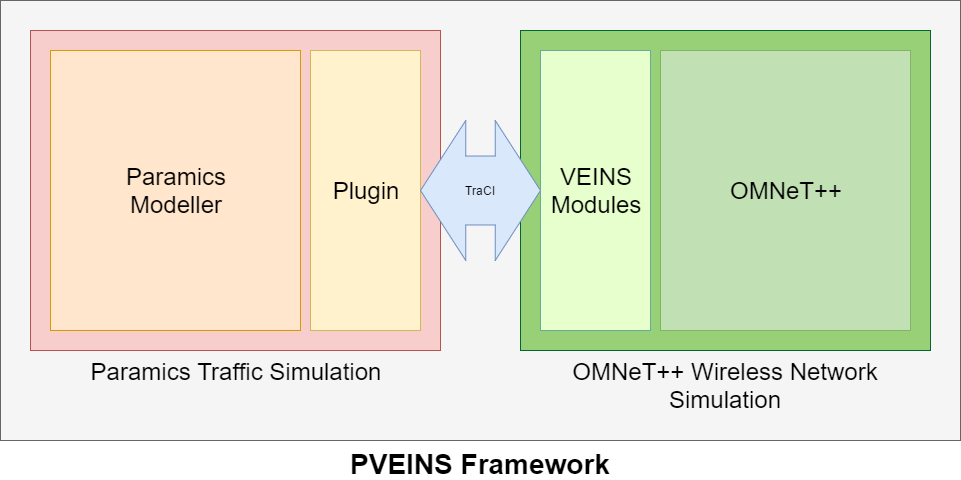
\includegraphics[width=\linewidth]{figuras/PVEINSArch.png}
    \caption{Visión macroscópica del framework; el plugin desarrollado actúa como una interfaz entre TraCI y Paramics.}
    \label{fig:pveins_genarch}
\end{figure}

A nivel más microscópico, la arquitectura del \emph{framework} se desarrolló en dos versiones distintas, la primera de éstas siendo descartada al realizar las pruebas de validación del proyecto. A continuación, se describirán brevemente estas dos iteraciones del diseño del software, destacando principalmente las razones del descarte de la versión preliminar.

\subsubsection{Arquitectura preliminar}

Originalmente, el \emph{framework} se implementó como un hilo de ejecución (un \emph{thread}) paralelo a Paramics. La principal ventaja de este diseño era evitar el bloqueo de la interfaz del simulador al encontrarse el servidor TraCI bloqueado esperando mensajes entrantes en el \emph{socket}. 

Un diagrama de la arquitectura general de esta implementación puede observarse en la figura \ref{fig:ptraci_arch}. Al iniciarse Paramics, el \emph{plugin} inicializaba el servidor en un \emph{thread} paralelo; el servidor luego se enlazaba a un \emph{socket} TCP y se bloqueaba en espera de mensajes entrantes desde un cliente TraCI (en nuestro caso, VEINS). Al recibir una serie de comandos TraCI, el servidor los interpretaba, comunicándose con Paramics a través de su API, obteniendo datos y modificando el estado de la simulación. El servidor interpretaba todos los comandos en un mensaje TraCI antes de enviar todos los mensajes de respuesta correspondientes en un único mensaje TraCI.

Esta arquitectura funcionaba de manera eficiente y permitía la ejecución de la simulación de Paramics completamente sin la intervención del usuario (ya que el \emph{thread} mismo del \emph{plugin} era capaz de llamar el método de inicio de simulación). 

Sin embargo, al comenzar a realizar pruebas con redes de tamaño más extenso se presentó un problema imprevisto, y -- a la larga -- irreparable sin acceso al código fuente de Paramics. El problema radicaba en la función de avance de simulación definido en la API de Paramics, \texttt{qps\_GUI\_runSimulation()}, la cual, como se descubrió más tarde, también actualiza la interfaz gráfica de el modelador de Paramics a través de llamados a la librería Qt4 \cite{qt}. Estos llamados no son \emph{thread-safe}\footnote{Es decir, no incluyen medidas para asegurar el acceso exclusivo de recursos a un sólo \emph{thread}.}, y en redes grandes de Paramics generan \emph{data races} al ser invocados desde un \emph{thread} paralelo al principal del simulador. Esto finalmente generaba corrupción de memoria en el motor gráfico (principalmente, lecturas de direcciones inválidas de memoria), lo cual causaba un error fatal en la simulación.

Se estudiaron múltiples maneras de resolver este problema manteniendo la estructura paralela del \emph{plugin} sin éxito, ya que la única manera confiable de forzar un avance de la simulación desde el \emph{plugin} es a través de la función anteriormente mencionada. Se decidió entonces abordar el problema desde un ángulo distinto, enfoque que se discutirá en la siguiente sección.

\begin{figure}[]
    \centering
    \begin{sequencediagram}
    \newthread{D}{OMNeT++}{}
    \newinst[1]{A}{VEINS}{}
    \newinst[3]{B}{Plugin (TraCIServer)}{}
    \newthread[2]{C}{Paramics}{}
    
    \begin{messcall}{C}{run()}{B}
        \postlevel
        \begin{call}{B}{waitForCommands()}{B}{}
        \end{call}
    \end{messcall}
    
    \begin{call}{D}{Solicitud}{A}{Resultado}
    
        \begin{call}{A}{Comando TraCI}{B}{Respuesta TraCI}
            \begin{call}{B}{parseCommand()}{B}{sendResponse()}
                \postlevel
                \begin{call}{B}{API Paramics}{C}{Datos}
                \end{call}
                \postlevel
            \end{call}
        \end{call}
    \end{call}
\end{sequencediagram}
    \caption{Arquitectura preliminar}
    \label{fig:ptraci_arch}
\end{figure}

\subsubsection{Arquitectura final} \label{sec:architecture:final}

El problema presentado por la incompatibilidad de \texttt{qps\_GUI\_runSimulation()}, función de avance de simulación de la API de Paramics, con múltiples \emph{threads} implicó la necesidad de reevaluar la arquitectura general del \emph{framework} en su totalidad. Se decidió descartar la idea de un \emph{thread} paralelo para el servidor, y se implementó un esquema secuencial de interpretación de mensajes TraCI, utilizando \emph{loops} bloqueantes para controlar la ejecución de pasos de simulación.

Esta arquitectura puede visualizarse en la figura \ref{fig:ptraci_arch2}. Al principio de cada paso de simulación, el simulador invoca la función \texttt{qpx\_CLK\_startOfSimLoop()}, definida en el \emph{plugin}, antes de realizar cualquier otra acción. Esta función a su vez invoca el método \texttt{preStep()} del servidor, dentro del cual se ejecuta un \emph{loop} de interpretación de comandos TraCI (y de envío de respuestas a éstos). Este \emph{loop} se interrumpe al recibir un mensaje de paso de simulación, retornando así de \texttt{preStep()} y \texttt{qpx\_CLK\_startOfSimLoop()}, y liberando al simulador para que realice su procedimiento interno de avance de simulación. 

Luego de realizar el avance de simulación, Paramics invoca la función \texttt{qpx\_CLK\_endOfSimLoop()}, también definida en el \emph{plugin}. Esta invoca a su vez el método \texttt{postStep()} del servidor, el cual se encarga de realizar la recolección de datos post-paso de simulación, de terminar de interpretar eventuales comandos recibidos previo al paso de simulación y de enviar respuestas pendientes al cliente. Finalmente, esta función retorna el control de la ejecución a Paramics, y el ciclo comienza nuevamente.

Mediante esta arquitectura se logró eliminar por completo el problema presentado por \texttt{qps\_GUI\_runSimulation()}, obteniendo incluso una leve mejora en rendimiento respecto al diseño antiguo, dado que, ya que todo corre en un sólo \emph{thread}, se evita el uso de elementos de sincronización, los cuales pueden agregar \emph{overhead} al procedimiento.

Este nuevo diseño presenta una única desventaja: es necesario el inicio de la simulación de manera manual por parte del usuario, luego de lo cual funciona de manera autónoma. Esto ya que no existe manera de iniciar el \emph{loop} de simulación de Paramics a través de la API sin recurrir a \emph{threads}.

Finalmente, se debe notar que dada la representación en tiempo discreto de los pasos de simulación, el avance de esta en muchos casos no alcanza exactamente el tiempo deseado. Si definimos el paso de simulación como $\triangle T$, el instante de tiempo en que se recibe el comando de avance como $T_{i}$ y el instante de tiempo objetivo $T_{o}$, la simulación se avanzará un número $n \in \mathbb{N}$ de pasos, tal que

\[ T_{i} + (n \times \triangle T) = T_{f} \]
\[ T_{i} + ((n - 1) \times \triangle T) = T_{f}' \]
\[ T_{f} \geq T_{o} \]
\[ T_{f}' < T_{o} \]

En otras palabras, la simulación se avanzará el mínimo número de pasos tal que el tiempo final es \emph{igual o mayor} al instante de tiempo objetivo. Esto es para asegurar que se ejecuten todas las acciones que dependan del tiempo de simulación por lo menos hasta dicho instante.

\begin{figure}[]
    \centering
    \begin{sequencediagram}
    \newthread{B}{Paramics + Plugin}{}
    \newthread[7]{A}{OMNeT++/VEINS}{}

    \begin{sdblock}{Loop de simulación}{}
        \postlevel
        \begin{call}{B}{\texttt{qpx\_CLK\_startOfSimLoop()}}{B}{}
            \begin{sdblock}{Loop pre-simulación}{}
                \begin{call}{B}{\texttt{server->preStep()}}{B}{Comando: Paso de Simulación}
                    \begin{call}{A}{Mensajes TraCI}{B}{Respuestas TraCI}
                        \postlevel
                    \end{call}
                \end{call}
            \end{sdblock}
        \end{call}
        \begin{sdblock}{Paso de simulación}{}
            \postlevel
            \postlevel
            \begin{call}{B}{\begin{minipage}{8cm}
                        Actualización de estado:
                        \begin{itemize}
                            \item Salida y llegada de vehículos
                            \item Modificación de velocidades y rutas
                        \end{itemize}
                \end{minipage}}{B}{}
            \end{call}
        \end{sdblock}
        \postlevel
        \begin{call}{B}{\texttt{qpx\_CLK\_endOfSimLoop()}}{B}{}
            \begin{sdblock}{Loop post-simulación}{}
                \begin{call}{B}{\texttt{server->postStep()}}{B}{Fin de Comandos}
                    \begin{call}{A}{Mensajes TraCI}{B}{Respuestas TraCI}
                        \postlevel
                    \end{call}
                \end{call}
            \end{sdblock}
        \end{call}
    \end{sdblock}
\end{sequencediagram}
    \caption{Arquitectura final del \emph{framework}}
    \label{fig:ptraci_arch2}
\end{figure}
\newpage
\section{Metodología de desarrollo} \label{sec:metodologia}

El desarrollo del \emph{plugin} se llevó a cabo de manera iterativa, implementando funcionalidades esenciales en primera instancia, y luego construyendo sobre esta base, cuidando en cada paso de no pasar a llevar las funcionalidades previamente implementadas y perfeccionando implementaciones anteriores. El orden de desarrollo de las funcionalidades fue cuidadosamente planeado, tomando en cuenta que en muchos casos se requería un orden específico de implementación de funcionalidades; \emph{e.g.} era imperativo el desarrollo de la funcionalidad de obtención de variables de vehículos antes de poder implementar suscripciones, ya estas últimas dependen de la funcionalidad de la primera. Las etapas generales de desarrollo que se siguieron fueron:

\begin{enumerate}
    \item En primer lugar, se desarrolló la base de comunicaciones del \emph{framework}, es decir, comunicación con el \emph{socket}, recepción e interpretación de mensajes. 
    
    \item A continuación, se implementó la funcionalidad esencial de control de simulación (los comandos presentados en la sección \ref{sec:comandos:controlsim}), con el fin de poder establecer una primera conexión con un cliente TraCI y simplemente ejecutar una simulación sin otros comandos. 
    El protocolo define un ``\emph{handshake}'' consistente en la verificación de versiones de TraCI compatibles entre cliente y servidor, por lo que el correcto funcionamiento del comando de obtención de versión fue prioridad en esta etapa.
    
    \item En tercer lugar se implementaron los comandos de obtención de variables de la simulación. Teniendo ya la base de comunicaciones funcionando, la implementación de éstos fue mucho más directa.
    
    \item Cuarto, sobre la implementación de los comandos de obtención de variables, se desarrollaron los distintos tipos de suscripciones disponibles.
    
    \item Finalmente, en última instancia, se desarrollaron los comandos de modificación de estados, ya que éstos necesariamente requerían una fundación sólida dada su relativa complejidad.
\end{enumerate}

Cabe destacar que, pese a la cuidadosa planificación realizada previa al desarrollo del \emph{framework} (y como siempre sucede en el desarrollo de \emph{software}), en muchas oportunidades fue necesario volver a un paso anterior para rediseñar o mejorar una implementación. El principal ejemplo de ésto es el rediseño de la arquitectura general del \emph{plugin}, detallado en la sección \ref{sec:architecture}, el cual implicó el rediseño y posterior reimplementación de gran parte de las etapas 1 (base de comunicaciones) y 2 (funcionalidad de control de simulación) del \emph{plugin}.

En términos de control de versiones y manejo del historial del desarrollo se escogió utilizar el sistema \emph{git} \autocite{git}, dada su popularidad, extenso soporte y documentación y la familiaridad del memorista con este sistema. El servicio de \emph{hosting} específico escogido para sistema fue \emph{GitHub} \autocite{github}; el código fuente del proyecto puede encontrarse en el perfil personal del autor \autocite{molguin_github}, en el repositorio \autocite{pveins_github}.

\section{Funcionalidad Implementada}

El protocolo TraCI define más de 30 comandos distintos, cada uno con una gran cantidad de variables y parámetros asociados (ver apéndice \ref{anex:traci} para una descripción más detallada del funcionamiento de este protocolo). Implementar esta gran cantidad de funcionalidades no hubiese sido factible, por lo que se escogió un subconjunto acotado de éstas a implementar, considerando en específico aquellos comandos esenciales para simulaciones de ITS.

\subsection{Comandos Implementados} \label{sec:comandos}

\subsubsection{Comandos de Control de Simulación}

\begin{itemize}
    \begin{multicols}{2}
        \mcitem{\texttt{0x00} Obtención de Versión}
        \mcitem{\texttt{0x02} Avance de Simulación}
        \mcitem{\texttt{0xff} Cierre de Conexión}
    \end{multicols}
\end{itemize}

\subsubsection{Comandos de Obtención de Variables}

\begin{description}[style=multiline]
    
    \item[\texttt{0xa4}] Variables de vehículos
    \begin{multicols}{2}
        \begin{itemize}
            \mcitem{\texttt{0x00} Lista de vehículos activos en la red}
            \mcitem{\texttt{0x01} Número de vehículos activos en la red}
            \mcitem{\texttt{0x36} Inclinación actual}
            \mcitem{\texttt{0x39} Posición actual (3D)}
            \mcitem{\texttt{0x40} Velocidad actual}
            \mcitem{\texttt{0x42} Posición actual (2D)}
            \mcitem{\texttt{0x43} Ángulo actual}
            \mcitem{\texttt{0x44} Largo}
            \mcitem{\texttt{0x4d} Ancho}
            \mcitem{\texttt{0x4f} Tipo de vehículo}
            \mcitem{\texttt{0x50} Calle actual}
            \mcitem{\texttt{0x51} Identificador de pista actual}
            \mcitem{\texttt{0x52} Índice de pista actual}
            \mcitem{\texttt{0xbc} Altura}
        \end{itemize}
    \end{multicols}
    
    \item[\texttt{0xa5}] Variables de tipos de vehículos
    \begin{multicols}{2}
        \begin{itemize}
            \mcitem{\texttt{0x00} Lista de tipos definidos}
            \mcitem{\texttt{0x01} Número de tipos definidos}
            \mcitem{\texttt{0x41} Velocidad máxima}
            \mcitem{\texttt{0x44} Largo}
            \mcitem{\texttt{0x46} Aceleración máxima}
            \mcitem{\texttt{0x47} Deceleración máxima}
            \mcitem{\texttt{0x4d} Ancho}
            \mcitem{\texttt{0xbc} Altura}
        \end{itemize}
    \end{multicols}
    
    \item[\texttt{0xa6}] Variables de rutas
    \begin{multicols}{2}
        \begin{itemize}
            \mcitem{\texttt{0x00} Lista de rutas definidas}
            \mcitem{\texttt{0x01} Número de rutas definidas}
            \mcitem{\texttt{0x54} Arcos (calles) componentes de la ruta}
        \end{itemize}
    \end{multicols}
    
    \item[\texttt{0xa8}] Variables de polígonos (edificios y estructuras)
    \begin{multicols}{2}
        \begin{itemize}
            \mcitem{\texttt{0x00} Lista de polígonos}
            \mcitem{\texttt{0x01} Número de polígonos}
        \end{itemize}
    \end{multicols}
    
    Cabe notar que Paramics no maneja edificios en sus simulaciones, al menos no edificios accesibles a través de la API de programación, por lo que estos métodos se implementaron de manera que reportan siempre 0 polígonos en la simulación.
    
    \item[\texttt{0xa9}] Variables de nodos (intersecciones) de la red
    \begin{multicols}{2}
        \begin{itemize}
            \mcitem{\texttt{0x00} Lista de intersecciones}
            \mcitem{\texttt{0x01} Número de intersecciones}
            \mcitem{\texttt{0x42} Posición de la intersección}
        \end{itemize}
    \end{multicols}
    
    \item[\texttt{0xaa}] Variables de arcos (calles) de la red
    \begin{multicols}{2}
        \begin{itemize}
            \mcitem{\texttt{0x00} Lista de calles}
            \mcitem{\texttt{0x01} Número de calles}
        \end{itemize}
    \end{multicols}
    
    \item[\namedlabel{item:simvars}{\texttt{0xab}}] Variables de Simulación
    \begin{multicols}{2}
        \begin{itemize}
            \mcitem{\texttt{0x70} Tiempo de simulación}
            \mcitem{\texttt{0x73} Número de vehículos liberados a la red en el último paso de simulación}
            \mcitem{\texttt{0x74} Lista de vehículos liberados a la red en el último paso de simulación}
            \mcitem{\texttt{0x79} Número de vehículos que han llegado a su destino en el último paso de simulación}
            \mcitem{\texttt{0x7a} Lista de vehículos que han llegado a su destino en el último paso de simulación}
            \mcitem{\texttt{0x7b} Tamaño del paso de simulación}
            \mcitem{\texttt{0x7c} Coordenadas de los límites de la red vehicular}
        \end{itemize}
    \end{multicols}
    
    Las variables \texttt{0x75}, \texttt{0x76}, \texttt{0x77} y \texttt{0x78}, correspondientes a los números y listas de vehículos que comienzaron y terminaron de teletransportarse en el último paso de simulación, así como las variables \texttt{0x6c}, \texttt{0x6d}, \texttt{0x6e} y \texttt{0x6f}, las cuales corresponden a números y listas de vehículos que comenzaron y terminaron de estar estacionados, fueron implementadas ``parcialmente''. En estricto rigor, los mecanismos subyacentes no se implementaron porque no se consideraron críticos, pero se implementó una respuesta \emph{dummy} de 0 vehículos para asegurar su funcionamiento con VEINS.
    
\end{description}

\subsubsection{Comandos de modificación de estado}\label{sec:mod_state}

\begin{description}[style=multiline]
    \item [\texttt{0xc4}] Variables de vehículo
    \begin{multicols}{2}
        \begin{itemize}
            \mcitem{\texttt{0x13} Cambio de pista}
            \mcitem{\texttt{0x14} Cambio de velocidad (lineal)}
            \mcitem{\texttt{0x40} Cambio de velocidad (instantáneo)}
            \mcitem{\texttt{0x41} Cambio de velocidad máxima}
            \mcitem{\texttt{0x45} Coloreado}
            \mcitem{\texttt{0x57} Cambio de ruta (a una lista de arcos otorgada por el cliente)}
            
        \end{itemize}
    \end{multicols}
\end{description}
%\section{Organización Lógica del Código}

El código del \emph{plugin} se separó en una serie de módulos lógicos que encapsulan y abstraen cada uno una categoría de funcionalidades de la interfaz con TraCI. De esta manera, se logró una separación lógica de las funcionalidades implementadas, y se simplifican futuras extensiones al código. La organización en archivos de éstos módulos puede observarse en la figura \ref{fig:dirtree}.

Cabe notar también que se utilizó el \emph{namespace} \texttt{traci\_api} para agrupar los elementos propios del framework. 

\begin{figure}[h]
    \dirtree{%
        .1 src/.
        .2 plugin.c\DTcomment{Archivo de inicio del \emph{plugin}}.
        .2 TraCIAPI/\DTcomment{Implementación de la API}.
        .3 Constants.h\DTcomment{Constantes utilizadas en el sistema}.
        .3 Exceptions.h\DTcomment{Excepciones propias del framework}.
        .3 Network.\{cpp/h\}\DTcomment{Métodos de interacción con la red vehicular}.
        .3 Simulation.\{cpp/h\}\DTcomment{Métodos de interacción con la simulación vehicular}.
        .3 Subscriptions.\{cpp/h\}\DTcomment{Suscripciones TraCI}.
        .3 TraCIServer.\{cpp/h\}\DTcomment{Módulo principal, manejo de conexiones TraCI}.
        .3 Triggers.\{cpp/h\}\DTcomment{Operaciones disparadas (temporales o situacionales)}.
        .3 Utils.\{cpp/h\}\DTcomment{Funciones auxiliares y de conveniencia}.
        .3 VehicleManager.\{cpp/h\}\DTcomment{Métodos de interacción con vehículos}.
        .2 shawn/\DTcomment{Archivos externos}.
        .3 socket.\{cpp/h\}\DTcomment{Manejo simplificado de \emph{sockets} TCP}.
        .3 storage.\{cpp/h\}\DTcomment{Manejo simplificado de paquetes de datos}.
    }
    \caption{Estructura de archivos del código fuente del framework.}
    \label{fig:dirtree}
\end{figure}

\subsection{plugin.c}\label{sec:plugin.c}

Si bien en estricto rigor no es un módulo del \emph{framework}, merece ser mencionado al ser el archivo principal del \emph{plugin} desarrollado. En este archivo se definen las funciones de extensión y \emph{override} (prefijos \texttt{QPX} y \texttt{QPO}, ver apéndice \ref{anex:paramics_api} para un detalle sobre la API de Paramics) a ser invocadas por Paramics. A continuación se describirán brevemente las más importantes de estas funciones, mientras que el archivo \texttt{plugin.c} puede estudiarse en su totalidad en el código \ref{code:pluginc} en los anexos.

\subsubsection{\texttt{void qpx\_NET\_postOpen()}}\label{sec:qpx_postopen}

Invocada inmediatamente luego de que Paramics carga la red y el \emph{plugin}, esta función inicializa el servidor TraCI. Para esto, crea un \emph{thread} donde corre una función auxiliar \texttt{runner\_fn()}, la cual se encarga de:

\begin{enumerate}
    \item Obtener el puerto en el cual esperar conexiones entrantes desde los parámetros de ejecución de Paramics. De no haberse especificado puerto, utiliza uno por defecto.
    \item Inicializar un objeto \texttt{TraCIServer} (ver sección \ref{sec:traciserver}) encargado de las conexiones entrantes en el puerto anteriormente definido.
\end{enumerate}

\subsubsection{\texttt{void qpx\_CLK\_startOfSimLoop()} y \texttt{void qpx\_CLK\_endOfSimLoop()}}

Estas funciones se ejecutan antes y después de cada paso de simulación respectivamente, y llaman a los procedimientos correspondientes en el servidor, los método \texttt{preStep()} y \texttt{postStep()}. Ver sección \ref{sec:traciserver} para más detalle sobre estos métodos y el avance de simulación en general.

\subsubsection{\texttt{void qpx\_VHC\_release(\dots)} y \texttt{void qpx\_VHC\_arrive(\dots)}}

\texttt{qpx\_VHC\_release(VEHICLE* vehicle)} es invocada por Paramics cada vez que un vehículo es liberado a la red de transporte. Simplemente se encarga de notificar al \texttt{VehicleManager} (ver sección \ref{sec:vehiclemanager}) para su inclusión en el modelo interno del \emph{plugin}.

Por otro lado, \texttt{qpx\_VHC\_arrive(VEHICLE* vehicle, LINK* link, ZONE* zone)} es invocada cuando un vehículo alcanza su destino final, y notifica al \texttt{VehicleManager} para eliminar el vehículo en cuestión de la representación interna.

\subsubsection{\texttt{int qpo\_RTM\_decision(\dots)}}\label{sec:plugin.c:decision}

Esta función de \emph{override} es llamada por el núcleo de simulación de Paramics cada vez que un vehículo necesita evaluar su elección de ruta, y debe retornar el índice de la siguiente salida que el vehículo debe tomar (o 0 si se desea mantener la ruta por defecto). En el \emph{plugin} se utiliza para aplicar rutas personalizadas otorgadas por el cliente TraCI.

\subsubsection{\texttt{void qpx\_VHC\_transfer(\dots)}}

Este método es ejecutado por Paramics cada vez que un vehículo pasa de una calle a otra, y se utiliza para determinar si es necesario recalcular la ruta del vehículo en cuestión.

\subsubsection{\texttt{float qpo\_CFM\_leadSpeed(\dots)} y \texttt{float qpo\_CFM\_followSpeed(\dots)}}\label{sec:plugin.c:speed}

Estas funciones se invocan en cada paso de simulación para cada vehículo en la simulación de tráfico de Paramics -- \texttt{leadSpeed()} se invoca para aquellos vehículos que no tienen otro vehículo delante, mientras \texttt{followSpeed()} es invocada los vehículos que se encuentran detrás de otro.

Estas funciones deben retornar la rapidez que se le deberá aplicar al vehículo en cuestión en el siguiente paso de simulación. En el \emph{framework}, se utilizan para aplicar cambios de velocidad dictados por comandos TraCI.

\subsection{TraCIServer}\label{sec:traciserver}

Implementa el funcionamiento base del servidor TraCI. Es el primer módulo como tal en inicializarse, y tiene como funciones:

\begin{enumerate}
    \item Asociarse a un \emph{socket} TCP, y esperar una conexión de un cliente TraCI.
    \item Mientras exista una conexión abierta, recibir e interpretar comandos TraCI entrantes.
    \item Enviar mensajes de estado y respuesta a comandos TraCI.
    \item Al recibir un comando de cierre, finalizar la simulación y cerrar el \emph{socket}.
\end{enumerate}

El módulo en cuestión se implementó como una clase de C++ en los archivos \href{https://github.com/molguin92/paramics_traci/blob/master/src/TraCIAPI/TraCIServer.h}{/src/TraCIAPI/TraCIServer.h} y \href{https://github.com/molguin92/paramics_traci/blob/master/src/TraCIAPI/TraCIServer.cpp}{/src/TraCIAPI/TraCIServer.cpp}, y se crea una instancia en el archivo \href{https://github.com/molguin92/paramics_traci/blob/master/src/plugin.c}{plugin.c}.

Cabe destacar que para facilitar el uso de \emph{sockets} y la obtención y envío de datos a través de éstos, se utilizaron las clases \texttt{tcpip::Socket} y \texttt{tcpip::Storage}, definidas en los archivos \href{https://github.com/molguin92/paramics_traci/blob/master/src/shawn/socket.h}{src/shawn/socket.\{cpp/h\}} y \href{https://github.com/molguin92/paramics_traci/blob/master/src/shawn/storage.h}{src/shawn/storage.\{cpp/h\}}. \texttt{tcpip::Socket} abstrae el funcionamiento de un \textit{socket} TCP, y provee métodos de conveniencia que permiten leer y escribir mensajes TraCI completos como objetos \texttt{tcpip::Storage}. Estos a su vez proveen métodos para escribir y leer todo tipo de variables en dichos mensajes, sin la necesidad de hacer la conversión manual a bytes.

Estos archivos no fueron desarrollados por el memorista, sino que fueron obtenidos desde el código fuente de SUMO \footnote{Fuente SUMO: \url{https://github.com/planetsumo/sumo/tree/master/sumo/src/foreign/tcpip}. Debe notarse que, a su vez, los creadores de SUMO originalmente obtuvieron dichos archivos del código fuente del simulador de eventos discretos para redes de sensores \emph{SHAWN} \cite{kroller2005shawn}. Su fuente original se encuentra en \url{https://github.com/itm/shawn/tree/master/src/apps/tcpip}}, distribuidos bajo una licencia BSD\footnote{Licencia clases \texttt{tcpip::Socket} y \texttt{tcpip::Storage}: \url{http://sumo.dlr.de/wiki/Libraries_Licenses\#tcpip_-_TCP.2FIP_Socket_Class_to_communicate_with_other_programs}}.

A continuación se detalla la implementación de las funcionalidades anteriormente mencionadas.

\subsubsection{Inicio de conexión TraCI}

Como se mencionó en la sección \ref{sec:qpx_postopen}, al iniciarse el \emph{plugin} se crea un nuevo \emph{thread}, en el cual se crea una instancia de un objeto de la clase \texttt{TraCIServer}, al cual se le invoca su método \texttt{waitForConnection()} (código \ref{cod:traciserver_waitforconnection}).

\lstinputlisting[float=t, style=CPP, label={cod:traciserver_waitforconnection}, caption={Rutina de inicio de conexión.}]{codigo/traciserver_waitforconnection.cpp}
%\minipagelisting{codigo/traciserver_run.cpp}{Rutina de inicio de conexión.}{cod:traciserver_run}

Este método es simple: imprime información pertinente sobre el \emph{plugin} en la ventana de información de Paramics, y luego espera a recibir una conexión entrante. Es además el único del \emph{framework} que corre en un \emph{thread} paralelo a Paramics en la arquitectura final. Se decidió implementarlo de esta manera para que el inicio de Paramics fuera más fluido y no se bloqueara la interfaz mientras el servidor espera una conexión desde un cliente TraCI.

\subsubsection{Recepción e interpretación de comandos entrantes}

Como se explicó en la sección \ref{sec:architecture:final}, la interpretación de comandos entrantes y el avance del \emph{loop} de simulación se realizan en dos etapas; una previa al paso de simulación y una posterior a éste. Los métodos encargados de esto son \texttt{preStep()} y \texttt{postStep()}, los cuales se detallarán a continuación.

\subsubsection{\texttt{preStep()}}

El método \texttt{preStep()} es invocado por Paramics al principio de cada iteración del \emph{loop} de simulación, antes de ejecutar cualquier otra función. Este método se encarga de recibir mensajes nuevos entrantes a través del \emph{socket} desde el cliente TraCI, e interpreta los comandos dentro de un \emph{loop}. La implementación de éste método puede observarse en los apéndices, código \ref{cod:traciserver_prestep}.

Nótese que \texttt{preStep()} continuamente interpreta, ejecuta y responde a comandos, y sólo retorna al recibir un comando de avance de simulación. De esta manera, retorna el control de la ejecución a Paramics, y el simulador mismo se encarga de realizar el paso de simulación.

En términos de la interpretación de los mensajes, al recibir datos entrantes, el \emph{socket} retorna un objeto \texttt{tcpip::Storage} con el mensaje completo. Luego, en un \emph{loop} adicional, este mensaje se separa en sus comandos TraCI constituyentes, copiando la información perteneciente a cada comando en otro objeto \texttt{tcpip::Storage} temporal. Este objeto se entrega como parámetro al método \texttt{parseCommand()} para la interpretación del comando, luego de lo cual se limpia y se vuelve a utilizar para el siguiente comando.

Finalmente, interpretados todos los comandos, se envía la respuesta al cliente a través del mismo \emph{socket} y se limpian los objetos \texttt{tcpip::Storage} para su reutilización en una nueva iteración del \emph{loop} interno.

\subsubsection{postStep()} \label{sec:poststep}

Al recibir un comando de avance de simulación, \texttt{preStep()} inmediatamente retorna el control del flujo del programa a Paramics. El simulador entonces avanza la simulación, y luego ejecuta el método \texttt{postStep()} del servidor. Al igual que para \texttt{preStep()}, el código de éste método se puede encontrar en los anexos, código \ref{cod:traciserver_poststep}.

Este método tiene como fin la recopilación de las eventuales suscripciones existentes (ver sección \ref{sec:subs}), la interpretación de los comandos restantes en el último mensaje recibido antes del comando de avance de simulación y el envío de eventuales respuestas al cliente. Finalmente, este método retorna, y Paramics vuelve a iniciar una nueva iteración del \emph{loop} de simulación y a ejecutar \texttt{preStep()}.

Cabe notar que \texttt{postStep()} sólo se ejecuta inmediatamente después de la ejecución de un paso de simulación por parte de Paramics, y por ende no se ejecuta si nunca se recibe un comando de avance de simulación.

\subsubsection{Interpretación de comandos TraCI}

Como se mencionó anteriormente, la interpretación de los comandos se lleva a cabo en el método \texttt{parseCommand()}, el cual recibe un único comando encapsulado en un objeto \texttt{tcpip::Storage}. Este método tiene una única misión: interpretar el identificador del comando recibido y delegar su ejecución al método correspondiente de la clase \texttt{TraCIServer}. Su implementación es simple, y su esqueleto puede observarse en el código \ref{cod:traciserver_parsecommand}. En específico, el código del método se puede dividir en dos ramas de ejecución; en caso de comando de suscripción (cuyos identificadores se encuentran todos en el rango $[\texttt{0xd0}, \texttt{0xdb}]$) se extraen los parámetros de la suscripción y se invoca el método \texttt{addSubscription()} para la subsecuente validación y activación de ésta. Por el contrario, en caso de recibir un comando con identificador fuera de dicho rango, se procede a verificar su tipo mediante un \emph{switch}. Cada caso se relaciona con un comando y método específico a invocar, y en caso de no encontrarse el identificador en cuestión se notifica al cliente que el comando deseado no está implementado.

\begin{figure}[htpb]
    \lstinputlisting[style=CPP, label={cod:traciserver_parsecommand}, caption={Esqueleto de \texttt{parseCommand()}}]{codigo/traciserver_parsecommand.cpp}
\end{figure}

Se definieron una serie de métodos en \texttt{TraCIServer} encargados de obtener variables de la simulación o modificar el estado de ésta. El funcionamiento de los métodos es idéntico en todos los casos (a excepción de \texttt{cmdGetPolygonVar()}), y se limita al siguiente procedimiento (ver ejemplo en el código \ref{cod:traciserver_cmdgetvhcvar}):

\begin{enumerate}
    \item Obtener el valor desde el módulo apropiado (por ejemplo, \texttt{VehicleManager} para variables de vehículos, \texttt{Simulation} para variables de la simulación, etc.).
    \item En caso de error en la obtención de los datos (variable no implementada, objeto no existente, etc.), atrapar el error y determinar el curso de acción apropiado (por ejemplo, notificar al cliente).
    \item Finalmente, enviar un mensaje de estado de la solicitud y, en caso de éxito, el valor de la variable, al cliente.
\end{enumerate}

\begin{figure}[htpb]
    \lstinputlisting[style=CPP, label={cod:traciserver_cmdgetvhcvar}, caption={Ejemplo de método de obtención y empaquetado de variables en \texttt{TraCIServer}}]{codigo/cmdGetVhcVar.cpp}
\end{figure}

El caso de \texttt{cmdGetPolygonVar()} es especial. En TraCI, un polígono representa un edificio o una estructura presente en las cercanías de la simulación vehicular, la cual puede interferir con el modelo de comunicación inalámbrica en OMNeT++. Sin embargo, el modelador de Paramics no maneja elementos externos a la simulación de transporte, por lo que se decidió, en el caso de comandos de obtención de variables relacionadas, simplemente reportar que no existen polígonos en la simulación para simplificar la integración.


\subsubsection{Evaluación de suscripciones}\label{sec:subs}

Como se explicó en la sección \ref{sec:poststep}, luego de realizar un paso de avance de simulación, en \texttt{postStep()} se realiza la evaluación de las suscripciones activas en \texttt{TraCIServer}, mediante un llamado al método \texttt{processSubscriptions()}.

Como se detalla en el apéndice \ref{anex:traci}, el protocolo TraCI define 12 tipos de suscripciones a variables de objeto, las cuales comparten todas una estructura idéntica. Cada suscripción se caracteriza por su identificador de tipo y sus parámetros: tiempo de inicio, tiempo de fin, identificador del objeto y las variables a las cuales el cliente se ha suscrito. En la práctica, lo único que diferencia a las suscripciones entre sí son las categorías de objetos a las cuales están asociadas, y por ende, cómo obtener esos datos desde la implementación interna del \emph{plugin}. A raíz de esto, se decidió implementar un árbol de clases de C++ para representar las suscripciones en memoria (declarada e implementada en los archivos \href{https://github.com/molguin92/paramics_traci/blob/master/src/TraCIAPI/Subscriptions.h}{src/TraCIAPI/Subscriptions.h} y \href{https://github.com/molguin92/paramics_traci/blob/master/src/TraCIAPI/Subscriptions.cpp}{src/TraCIAPI/Subscriptions.cpp} respectivamente).

La raíz de éste árbol, la clase \texttt{VariableSuscription}, implementa la funcionalidad completa de evaluación y actualización de una suscripción en los métodos \texttt{handleSubscription()} y \texttt{updateSubscription()} (implementación completa de estos métodos en \ref{code:variablesubscription_main}), abstrayendo la obtención de datos específicos a cada tipo en los métodos \texttt{getObjectVariable()} y \texttt{getResponseCode()}. Estos métodos son \emph{virtuales} en la clase base, y son implementados por las clases derivadas, de manera que \texttt{TraCIServer} sólo necesita mantener un vector de variables del tipo base, las cuales se evalúan de manera polimórfica.

\begin{figure}[]
    \centering
    \begin{tikzpicture}% [ show background grid ]
    \begin{class}[text width=8cm]{VariableSubscription}{0 ,0}
        \operation{uint8\_t handleSubscription(\dots) \{\dots\}}
        \operation{uint8\_t updateSubscription(\dots) \{\dots\}}
        \operation[0]{virtual void getObjectVariable(\dots);}
        \operation[0]{virtual uint8\_t getResponseCode();}
    \end{class}
    
    \begin{class}[text width=7cm]{VehicleVariableSubscription}{4 ,-4}
        \inherit{VariableSubscription}
        \operation{void getObjectVariable(\dots) \{\dots\}}
        \operation{uint8\_t getResponseCode() \{\dots\}}
    \end{class}
    
    \begin{class}[text width=7cm]{SimulationVariableSubscription}{-4 ,-4}
        \inherit{VariableSubscription}
        \operation{void getObjectVariable(\dots) \{\dots\}}
        \operation{uint8\_t getResponseCode() \{\dots\}}
    \end{class}
\end{tikzpicture}
    \caption{Diagrama de herencia, \texttt{VariableSubscription}}
    \label{fig:cd_variablesub}
\end{figure}

En términos más simples, lo único que debe implementar una clase derivada de \texttt{VariableSubscription} para definir un nuevo tipo de suscripción son versiones propias de los métodos \texttt{getObjectVariable()} y \texttt{getResponseCode()}, ya que todo la demás funcionalidad de evaluación de suscripciones está ya implementada en la clase base. 

De esta manera, la evaluación en \texttt{TraCIServer} se simplifica, ya que la instancia sólo necesita mantener un vector con punteros a objetos de la clase base, dado que independiente de la implementación específica de los métodos \texttt{getObjectVariable()} y \texttt{getResponseCode()} de cada subclase, \texttt{handleSubscription()} es exactamente igual para todas (ver línea 7 en el código \ref{cod:traciserver_processsubs}). Además, esto facilita la extensión futura del software.

\begin{figure*}[h]
\lstinputlisting[style=CPP, label={cod:traciserver_processsubs}, caption={Rutina de evaluación de suscripciones en \texttt{TraCIServer}. \texttt{subs} es una variable de instancia de \texttt{TraCIServer} correspondiente a un vector de punteros \texttt{VariableSuscription*}, poblado de elementos de clases derivadas de \texttt{VariableSuscription}.}]{codigo/traciserver_processsubs.cpp}
\end{figure*}

\subsubsection{Creación de nuevas suscripciones}

Por otro lado, para crear nuevas suscripciones, \texttt{TraCIServer} debe considerar la categoría de objetos a la cual se está suscribiendo, e insertar un puntero a un objeto con el tipo correspondiente en la variable de instancia \texttt{subs}. Esto sucede al recibir un comando con un identificador correspondiente a una suscripción; los parámetros de la suscripción son extraídos y delegados al método \texttt{addSubscription()} (código \ref{cod:traciserver_parsecommand},línea 15). Este código puede estudiarse en su totalidad en el anexo \ref{chapter:anex_codes}, código \ref{code:addsub}, sin embargo, a continuación se explicará brevemente su funcionamiento con algunos extractos de código.

Como se comenta en la descripción del protocolo TraCI (apéndice \ref{anex:traci}), un comando de suscripción puede solicitar tanto la creación de una nueva suscripción como la actualización o cancelación de una ya existente. Esto se determina basado en si, al recibir el comando de suscripción, ya existe una suscripción asociada a dicha categoría y objeto. Esto es lo primero en verificarse en \texttt{addSubscription()}, mediante llamados al método \texttt{updateSubscription()} de cada suscripción ya existente en el servidor.

El funcionamiento de este método se detalla en el código \ref{code:variablesubscription_main}, a partir de la línea 70. Verifica si los parámetros recibidos corresponden a una suscripción ya existente, y retorna un byte cuyo valor representa el estado de la suscripción, valor interpretado por \texttt{addSubscription()} para determinar el curso de acción a tomar:
\begin{enumerate}
    \item \texttt{STATUS\_NOUPD}: Los parámetros entregados no corresponden a esta suscripción. \texttt{addSubscription()} sigue recorriendo las suscripciones restantes para verificar si corresponde a alguna ya existente.
    \item \texttt{STATUS\_UNSUB}: Los parámetros corresponden a una solicitud de cancelación de esta suscripción (categoría e identificador de objeto son los mismos, número de variables a suscribir es $0$). \texttt{addSubscription()} entonces procede a eliminar esta suscripción del vector \texttt{subs} en \texttt{TraCIServer} y liberar la memoria asignada al puntero.
    \item \texttt{STATUS\_ERROR}: Los parámetros corresponden a una actualización de esta suscripción (categoría e identificador de objeto son los mismos), pero sucedió un error en la actualización. \texttt{addSubscription()} escribe un mensaje de notificación al cliente y retorna.
    \item \texttt{STATUS\_OK}: Los parámetros corresponden a una actualización de esta suscripción (categoría e identificador de objeto son los mismos), y la actualización fue exitosa. \texttt{addSubscription()} escribe un mensaje de notificación al cliente y retorna.
\end{enumerate}

\begin{figure}[htpb]
    \lstinputlisting[style=CPP, label={code:addsub_upd},caption={Verificación de actualización en \texttt{addSubscription()}.}, linerange={7-38}]{codigo/traciserver_addsubscription.cpp}
\end{figure}


La segunda parte del método es más simple. De corresponder el comando a una solicitud de creación de una suscripción nueva, se verifica su tipo y dinámicamente se crea un objeto de la clase apropiada (como se explicó anteriormente, derivada de \texttt{VariableSubscription}). Finalmente, se verifica el correcto funcionamiento de la nueva suscripción mediante un llamado a su método \texttt{handleSubscription()} y se notifica al cliente del resultado.

\begin{figure*}[h]
    \lstinputlisting[style=CPP, label={code:addsub_instance},caption={Creación de una nueva suscripción. Notar la instanciación polimórfica.}, linerange={56-70}]{codigo/traciserver_addsubscription.cpp}
\end{figure*}
    
%\begin{figure}
%    \centering
%    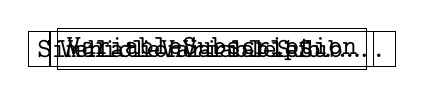
\begin{tikzpicture}
\tikzset{level distance=50pt}
\Tree [.\node[draw]{\texttt{VariableSubscription}};
[.\node[draw]{\texttt{VehicleVariableSub\dots}}; ]
[.\node[draw]{\texttt{SimulationVariableSub\dots}}; ]
[.{\dots} ]
]
\end{tikzpicture}
%    \caption{Árbol de herencia de suscripciones.}
%    \label{fig:subs_tree}
%\end{figure}

\subsubsection{Envío de resultados al cliente}

\texttt{TraCIServer} mantiene una variable de instancia \texttt{tcpip::Storage outgoing}, en la cual se almacenan los mensajes de estado y resultados de comandos TraCI. El envío de estos al cliente se efectúa al final de cada iteración del \emph{loop} en \texttt{preStep()} o, en el caso de recibir un comando de avance de simulación, en \texttt{postStep()}, enviando así conjuntamente las respuestas a todos los comandos obtenidos desde el cliente en el último paso de tiempo. Gracias a las clases \texttt{tcpip::Storage} y \texttt{tcpip::Socket} utilizadas, la operación de enviar los datos almacenados se reduce a una invocación del método \texttt{sendExact()} del objeto \texttt{tcpip::Socket}, la cual recibe un objeto \texttt{tcpip::Storage}, le adjunta una cabecera con su tamaño total y lo envía a través del \emph{socket} al cliente.

La escritura de datos en el almacenamiento saliente se implementó en dos métodos de \texttt{TraCIServer}; \texttt{writeStatusResponse()}, método de conveniencia para la escritura de mensajes de estado, y \texttt{writeToOutputWithSize()}, el cual recibe otro objeto de tipo \texttt{tcpip::Storage} que contiene el resultado de algún comando y escribe sus contenidos en \texttt{outgoing}, junto con una cabecera que indique su tamaño. Esto implicó también una decisión de diseño en términos de la comunicación de \texttt{TraCIServer} con los demás módulos del sistema. Se optó por realizar la mayor parte de esta comunicación mediante objetos de tipo \texttt{tcpip::Storage}, delegando la estructuración de los resultados de cada comando específico a los módulos responsables. De esta manera se aumenta la modularidad, ya que cada módulo sabe como escribir sus resultados de manera correcta, y \texttt{TraCIServer} sólo necesita asumir que recibirá un \texttt{tcpip::Storage} bien formateado como respuesta a los comandos.

\begin{figure*}[h]
\lstinputlisting[style=CPP, label={code:traciserver_writetooutput},caption={Escritura de datos en almacenamiento saliente.}]{codigo/traciserver_writetooutput.cpp}
\end{figure*}

\section{Simulation}\label{sec:simulation}

La principal funcionalidad de este módulo es abstraer y encapsular el acceso a los parámetros de la simulación vehicular de Paramics. Se implementó como una clase de C++ utilizando el patrón de diseño \emph{singleton}; esto quiere decir que sólo se permite la instanciación de un único objeto de este tipo en la ejecución del programa. Esto ya que, por razones lógicas, cada ejecución del \emph{plugin} está asociada a una única simulación en Paramics, y por ende no tiene sentido que pueda existir más de un objeto de acceso a ésta. Este patrón de diseño tiene además la ventaja que simplifica el acceso a la instancia global de la clase en el sistema, desde cualquier otro objeto u función.

\subsection{Obtención de variables}\label{sec:simulation:vars}

Las variables obtenibles desde este módulo son todas aquellas que se relacionan con la simulación como ente abstracto, enumeradas en el ítem \ref{item:simvars} de la sección \ref{sec:comandos}. La implementación de los métodos \texttt{packSimulationVariable()} y \texttt{getSimulationVariable()}, encargados de facilitar el acceso a las variables representadas por este módulo, pueden observarse en el código \ref{code:simvar} en los apéndices. Cabe destacar que los módulos \texttt{VehicleManager} y \texttt{Network} cuentan con métodos análogos \emph{muy} similares, por lo que no se incluirá el código de éstos últimos en el documento.

Se debe mencionar también la especial implementación de la obtención de algunas de las variables anteriormente mencionadas. En específico, las variables referentes a los vehículos que comenzaron o terminaron su viaje en el último paso de simulación son accesibles desde este módulo, pero su obtención fue implementada en el módulo \texttt{VehicleManager}. Esto ya que dicho módulo debe mantener una lista interna de todos los vehículos de la simulación en todo instante de tiempo, por lo que obtener estos valores era mucho más directo de implementar allá. Ver la sección sobre \texttt{VehicleManager}, \ref{sec:vehiclemanager}, para más detalles.

De las variables efectivamente implementadas en este módulo, vale destacar un par de detalles. En primer lugar, existe una diferencia entre cómo VEINS y OMNeT++ manejan el tiempo de simulación, y cómo lo hace Paramics; los primeros ocupan mili-segundos, mientras que este último ocupa segundos. Esto implicó realizar las respectivas conversiones necesarias.

En segundo lugar se hablará del comando de obtención de las coordenadas de los límites de la simulación. Este es de extrema importancia para VEINS, ya que con estos valores se crea el escenario de comunicación inalámbrica en OMNeT++; de ser erróneos, tarde o temprano la posición de un vehículo (representado por un nodo de comunicación en OMNeT++) quedará fuera del escenario, gatillando un error fatal en la simulación. 
Desafortunadamente, si bien la API de Paramics cuenta con un comando para, supuestamente, obtener estas coordenadas, por razones que no se lograron dilucidar, este comando retorna valores altamente erróneos (esto se verificó con múltiples redes de transporte).
Se debió entonces implementar el cálculo correcto de éstos límites en el módulo mismo, en el método, apropiadamente nombrado, \texttt{getRealNetworkBounds()} (expuesto en el código \ref{code:getrealnetworkbounds} en los anexos). Este cálculo se hace prácticamente a fuerza bruta, recorriendo todos los elementos que definen el alcance de la red (calles, intersecciones y zonas de emisión de vehículos), obteniendo sus coordenadas y luego obteniendo el rectángulo que las contiene (más un cierto margen de error).
Si bien este método no escala bien con redes más grandes, su impacto en la eficiencia del sistema se estimó como mínimo ya que se accede una única vez por simulación a este valor.

\section{VehicleManager}\label{sec:vehiclemanager}

El módulo más complejo y grande (en términos de líneas de código) del \emph{framework}. \texttt{VehicleManager} tiene como función abstraer el acceso a variables directamente relacionadas con los vehículos presentes en la simulación, mantener registros de dichos vehículos, y encargarse de ejecutar los diversos cambios de estado de éstos que puede solicitar el cliente (ver \ref{sec:mod_state}). Además, varios de éstos cambios de estado requieren acciones en múltiples instantes de tiempo (por ejemplo, el cambio de velocidad lineal, el cual se ejecuta durante un periodo de tiempo determinado), por lo que adicionalmente el módulo mantiene colas de eventos diferidos a ejecutar en instantes determinados.

Para la implementación de éste módulo, se utilizó nuevamente el paradigma de \emph{singleton}, por las mismas razones esgrimidas que para \texttt{Simulation}.

A continuación se tratará de detallar los aspectos más importantes de este módulo.

\subsection{Estado interno}\label{sec:internalstate}

Para simplificar muchas de las operaciones de obtención de variables y modificación de estados, el módulo mantiene un estado interno congruente con el estado de la simulación en Paramics. Para este fin se ocupan los llamados de la API de Paramics mencionados en la sección \ref{sec:plugin.c}.

Se utilizan las siguientes variables para almacenar información sobre el estado de la simulación en todo instante:

\begin{description}[]
    \item[\texttt{vehicles\_in\_sim}] \emph{Hashmap} que almacena el ID y un puntero a cada vehículo presente en la simulación. Se utiliza ya que Paramics no provee un método directo para obtener un puntero a un vehículo dada su ID, sino que es necesario buscarlo en la red. Este método elimina esa búsqueda y facilita además el conteo de vehículos en la simulación (basta con obtener la cantidad de pares \texttt{\{llave, valor\}} en el \emph{hashmap}). Se actualiza dinámicamente cada vez que ingresa un vehículo nuevo a la red, a través del llamado al método \texttt{vehicleDepart()} del presente módulo desde \texttt{plugin.c}.
    
    \item[\texttt{departed\_vehicles} y \texttt{arrived\_vehicles}] Vectores de punteros a vehículos, actualizados por Paramics a través de las funciones de extensión de la API \texttt{qpx\_VHC\_release()} y \texttt{qpx\_VHC\_arrive()} en \texttt{plugin.c} (ver sección \ref{sec:plugin.c}). Mantienen punteros a vehículos que iniciaron su viaje y que llegaron a su destino, respectivamente, en último paso de simulación. Se vacían al antes de cada paso.
    
    \item[\texttt{speed\_controllers}] Mapa que relaciona vehículos con controladores de velocidad (ver sección \ref{sec:speedoverride}), para efectuar cambios de velocidad dictados por el cliente TraCI.
    
    \item [\texttt{vhc\_routes}] Mapa para el manejo de cambios de ruta desde TraCI (ver sección \ref{sec:routeoverride}).
    
    \item[\texttt{lane\_set\_triggers}] \emph{Hashmap} utilizado para relacionar vehículos con eventuales comandos de cambio de pista (ver sección \ref{sec:laneoverride}).
\end{description}

\subsection{Obtención de variables}

La función más básica de \texttt{VehicleManager} es la de abstraer el acceso a las variables de simulación directamente relacionadas con vehículos y tipos de vehículos. Los principales métodos encargados de estas funcionalidades son \texttt{getVehicleVariable()} y \texttt{getVhcTypesVariable()}, respectivamente, aunque éstos por lo general son invocados por \texttt{packVehicleVariable()} y \texttt{packVhcTypesVariable()}, respectivamente, métodos que empaquetan los resultados en un \texttt{tcpip::Storage} para su fácil manejo. 

\texttt{getVehicleVariable()} y \texttt{getVhcTypesVariable()} son métodos relativamente simples, los cuales simplemente comparan el identificador de variable proporcionado como argumento y obtienen el valor solicitado mediante un llamado a alguna de los métodos auxiliares implementados para la obtención de variables. Dada su gran similitud con los métodos \texttt{packSimulationVariable()} y \texttt{getSimulationVariable()} ya presentados en la sección \ref{sec:simulation:vars}, dedicada a la obtención de variables desde el módulo \texttt{Simulation}, no se presentará la implementación de los métodos propios del presente módulo en el documento (ver código \ref{code:simvar} para un acercamiento a la implementación real de éstos).

\subsection{Modificación de estado de vehículos}

La segunda función de \texttt{VehicleManager} es la de ejecutar los comandos de modificación de estado y comportamiento de los vehículos en la simulación (ver sección \ref{sec:mod_state} para una lista de los comandos de este tipo que se implementaron). El método \texttt{setVehicleState()} es el encargado de la interpretación de comandos de cambio de estado, y su implementación es simple; determina el tipo de cambio de estado solicitado y si se encuentra implementado delega su ejecución al método correspondiente.

Dos de los comandos de cambio de estado implementados, \texttt{0x45 Coloreado} y \texttt{0x41 Cambio de velocidad máxima}, se ejecutan de manera directa a través de la API de Paramics. El resto requiere procedimientos más complejos, los cuales se describirán brevemente a continuación.

\subsubsection{Cambios de velocidad lineal e instantáneo}\label{sec:speedoverride}

Los comandos de cambio de velocidad de TraCI requieren un procedimiento especial ya que el efecto tiene debe aplicarse por un periodo mayor a un sólo paso de simulación, y por lo tanto es necesario un procedimiento que se encargue de mantener el efecto en el tiempo. Esto se implementó mediante la clase \texttt{traci\_api::BaseSpeedController} y sus derivadas.

\texttt{traci\_api::BaseSpeedController} define una clase compuesta únicamente de métodos virtuales, en base a la cual se construyen distintos tipos de controladores de velocidad. Como se comentó anteriormente, en la sección \ref{sec:internalstate}, \texttt{VehicleManager} mantiene un \emph{hashmap} que relaciona vehículos con controladores derivados de la clase anteriormente mencionada. Este mapa es accedido para cada vehículo, en cada paso de simulación por el método \texttt{speedControlOverride()} (a su vez, invocado por \texttt{qpo\_CFM\_followSpeed()} y \texttt{qpo\_CFM\_leadSpeed()} -- ver sección \ref{sec:plugin.c:speed}), el cual verifica si el vehículo en cuestión cuenta con un modificador de velocidad y aplica el cambio necesario. Además, cada controlador de velocidad cuenta con un método \texttt{repeat()} para verificar si debe seguir aplicándose en pasos de simulación futuros -- de no ser así, se elimina de la representación interna.

\lstinputlisting[style=CPP, label={cod:vehiclemanager_speedcontrol}, caption={Método de verificación de control de velocidad en VehicleManager. Verifica la existencia de un controlador personalizado de velocidad en \texttt{speed\_controllers} y luego guarda el resultado de la evaluación en la variable \texttt{speed}.}]{codigo/vehiclemanager_speedcontrol.cpp}

En la implementación final del \emph{framework} se definieron dos clases derivadas distintas de \texttt{traci\_api::BaseSpeedController}: \texttt{traci\_api::HoldSpeedController} y \texttt{traci\_api::LinearSpeedChangeController}, los cuales implementan, respectivamente, los cambios inmediatos y lineales de velocidad definidos en el protocolo TraCI. La implementación de éstos puede revisarse en los apéndices, código \ref{code:speedcontrollers}.

\subsubsection{Cambio de ruta}\label{sec:routeoverride}

TraCI cuenta con un comando \texttt{0x57 Cambio de Ruta} mediante el cual un cliente puede proveer un número de arcos (calles) que el vehículo en cuestión deberá seguir antes de reencaminarse a su destino original. Este comando es especial en que requiere invalidar el ruteo interno de Paramics para dicho vehículo mientras esté siguiendo la ruta otorgada por el cliente, lo cual puede durar un tiempo indefinido.

Para esto se definió entonces un método \texttt{rerouteVehicle()} en VehicleManager, el cual recibe un puntero a un vehículo y su calle actual, y retorna el índice de la siguiente salida que debe tomar -- en caso de tener una ruta personalizada, este método retornará el índice de la siguiente calle en la ruta, y de otro modo retorna 0, lo cual es interpretado por Paramics como una indicación a seguir la ruta dictada por el modelo interno.

\lstinputlisting[style=CPP, label={cod:vehiclemanager_reroute}, caption={Método de reruteo en VehicleManager, para vehículos con rutas dictadas por un cliente TraCI.}]{codigo/vehiclemanager_reroute.cpp}

Este método es invocado cada vez que un vehículo necesite evaluar su elección de ruta, a través de la función de extensión de la API de Paramics \texttt{int qpo\_RTM\_decision()} (ver sección \ref{sec:plugin.c:decision}).

Las rutas en sí se almacenan en la variable interna \texttt{vhc\_routes}; un \emph{hashmap} que relaciona vehículos con punteros a otro \emph{hashmap} más. Este segundo mapa es de tipo 
\texttt{<LINK*, int>}, relacionando cada arco en la ruta con un índice a la siguiente salida que deberá tomar el vehículo al encontrarse sobre ese arco. De esta manera no fue necesaria la implementación de una estructura de datos adicional para el almacenamiento de las rutas.

\subsubsection{Cambio de pista}\label{sec:laneoverride}

Finalmente, el comando de cambio de pista de TraCI también debe aplicarse por un tiempo determinado. Desafortunadamente, dadas ciertas limitaciones del modelo que utiliza Paramics para controlar la selección de pistas, este cambio no se pudo implementar como el cambio de ruta o el cambio de velocidad, dejando que la simulación de Paramics misma consultara la pista a tomar en el siguiente paso de simulación, sino que se debió implementar a ``fuerza bruta''.

Esto se logró mediante la implementación de la clase de métodos virtuales \texttt{traci\_api::}
\texttt{BaseTrigger} y su clase derivada \texttt{traci\_api::LaneSetTrigger}. \texttt{BaseTrigger} define una interfaz general para operaciones de ejecución periódica o diferida, y \texttt{LaneSetTrigger} representa una implementación de ésta interfaz para la ejecución constante de un cambio de pista por un tiempo definido.

\lstinputlisting[style=CPP, label={cod:lanesettrigger}, caption={Cambio de pista, implementado en \texttt{LaneSetTrigger}}]{codigo/lanesettrigger.cpp}

La ejecución de estos \emph{triggers} se maneja en el método \texttt{handleDelayedTriggers()} en \texttt{VehicleManager}, el cual es ejecutado al fin de cada paso de simulación. Cabe notar que si bien en la versión final del \emph{framework} sólo se implementó una clase derivada de \texttt{BaseTrigger}, el diseño polimórfico de la evaluación de los \emph{triggers} hace que en el futuro sea muy fácil la integración de nuevos procedimientos diferidos al sistema.

\lstinputlisting[style=CPP, label={cod:vehiclemanager_handledelayedtriggers}, caption={Manejo de \emph{triggers} para operaciones diferidas en \texttt{VehicleManager}}]{codigo/vehiclemanager_handledelayedtriggers.cpp}


\section{Otros módulos}\label{sec:miscmodules}

\subsection{Network}

El módulo \texttt{Network} encapsula el acceso a variables de elementos de la red, en particular, calles, intersecciones y rutas. Al igual que \texttt{VehicleManager} y \texttt{Simulation}, se implementó utilizando un \emph{singleton}. 

La implementación del módulo es muy simple, ya que sólo otorga acceso a elementos no modificables por el usuario. Sus métodos de acceso a variables, \texttt{getLinkVariable()}, \texttt{getJunctionVariable()} y \texttt{getRouteVariable()} son altamente similares al ya presentado \texttt{getSimulationVariable()} (código \ref{code:simvar}), y las únicas variables de instancia que mantiene son dos \emph{hashmaps}, las cuales se inicializan al momento de instanciarse el módulo:
\begin{description}
    \item [\texttt{route\_name\_map}] De tipo \texttt{<std::string, BUSROUTE*>}, relaciona nombres de rutas con punteros a éstas, para un acceso más directo y eficiente.
    
    \item [\texttt{route\_links\_map}] De tipo \texttt{<BUSROUTE*, std::vector<std::string>\@>}, asocia cada ruta con sus arcos constituyentes.
    
\end{description}

\lstinputlisting[style=CPP, label={cod:network_init}, caption={Constructor del módulo \texttt{Network}}]{codigo/network_init.cpp} 

\subsection{Utils}

En \texttt{Utils.\{cpp/h\}} se implementaron una serie de funciones de conveniencia:
\begin{itemize}
    \item \texttt{debugPrint()} e \texttt{infoPrint()}, para la escritura de mensajes a la ventana de información de Paramics, además de la salida de error y estándar respectivamente. 
    
    \item Las funciones \texttt{readTypeChecking<tipo>()}, las cuales reciben un elemento de tipo \texttt{tcpip::Storage} y leen el primer elemento contenido ahí, verificando que sea del tipo deseado. Estas funciones no fueron implementadas por el memorista, sino obtenidas del código fuente de SUMO.
    
    \item Las funciones \texttt{RGB2HEX()} y \texttt{HEX2RGB()}, para la conversión de colores entre ambas representaciones.
\end{itemize}

\subsection{Constants}

En el archivo de cabecera \texttt{Constants.h} se declararon una serie de constantes globales al sistema. No obstante, cada módulo maneja además un conjunto de constantes propias. Cabe notar que las constantes del \emph{framework} fueron definidas como \emph{variables constantes estáticas}, y no como \emph{definiciones del preprocesador}.

\begin{figure}[h]
    \centering
    \begin{minipage}{.49\linewidth}
        \begin{lstlisting}[style=CPP, numbers=none, frame=none, backgroundcolor=\color{white}]
        #define DUMMY_CONST 0x42
        \end{lstlisting}
    \end{minipage}
    \begin{minipage}{.49\linewidth}
        \begin{lstlisting}[style=CPP, numbers=none, frame=l, backgroundcolor=\color{white}]
        static const
        DUMMY_CONST = 0x42;
        \end{lstlisting}
    \end{minipage}
    \caption{Definición del preprocesador (izq.) \emph{vs} variable constante estática (der.).}
\end{figure}

La diferencia entre ambos métodos de definición radica en la interpretación que el \emph{toolchain} de compilación les da. Las \emph{definiciones del preprocesador} son interpretadas por el \emph{preprocesador}, antes de pasar por el compilador, y se ejecutan como simples reemplazos textuales en el código por el valor definido. Por otro lado, las variables constantes son tratadas como cualquier otra variable, y por ende cuentan con todas las propiedades de éstas. La decisión de utilizar este segundo método se tomó en base a que las variables constantes tienen la particularidad de estar restringidas a su \emph{scope} -- es decir, si se declaran por ejemplo dentro de un \emph{namespace} (como es el caso en \texttt{Constants.h}), su identificador no queda definido fuera de dicho entorno.
Esto es altamente deseable para futuras extensiones del \emph{framework}, \emph{e.g.} en el caso que se desee integrar con algún otro \emph{plugin} que ya cuente con sus propias constantes, ya que de esta manera se facilita la distinción de cual valor pertenece a qué parte del software. Por otro lado, las \emph{definiciones de preprocesador} tienen la ventaja de que no ocupan memoria en el programa final compilado (ya que los identificadores en el código se reemplazan directamente por el valor antes de compilarse el código); no obstante, dado que el número de constantes definidas es altamente acotado, el impacto en memoria de declararlas como variables del lenguage es negligible.

\subsection{paramics-launchd.py}

El archivo \texttt{paramics-launchd.py} corresponde a una versión modificada del \emph{script} de Python 2.7 \texttt{sumo-launchd.py} incluído con la distribución de VEINS, alterado para su funcionamiento con Paramics en vez de SUMO.

Este archivo funciona como un \emph{daemon} de ejecución del \emph{framework}, cuya labor es la de recibir conexiones entrantes desde clientes TraCI y preparar la simulación de Paramics para dar inicio a la simulación bidireccional. Su funcionamiento se detalla a continuación:

\begin{enumerate}
    \item El usuario inicia el \emph{script} en el \emph{host} donde se desea correr la simulación vehicular de Paramics. Gracias a la arquitectura cliente-servidor de VEINS (y por extensión, del presente proyecto), ambos simuladores pueden ejecutarse en equipos distintos (virtuales o físicos).
    
    \item Por defecto, el \emph{script} se asocia a un \emph{socket} en el puerto 9999 y espera conexiones TraCI entrantes.
    
    \item Por otro lado, el usuario inicia la simulación de VEINS en OMNeT++. Esta automáticamente se conecta con el puerto 9999 del \emph{host}, y le transfiere los contenidos de un archivo XML \texttt{paramics-launchd.xml}, definido por el usuario. Este archivo define parámetros de simulación como la red vehicular a utilizar y la \emph{semilla} deseada para la generación de valores pseudoaleatorios.
    
\lstinputlisting[style=myXML, label={cod:launchd_xml}, caption={Ejemplo de archivo XML de inicialización de la simulación.}, xleftmargin=\dimexpr-\csname @totalleftmargin\endcsname]{codigo/paramics_example.launchd.xml}
    
    \item Al recibir una conexión entrante junto con el archivo de configuración, \texttt{paramics-launchd.py} prepara el inicio de la simulación integrada siguiendo los siguientes pasos:
    
    \begin{enumerate}
        \item En primer lugar, encuentra un puerto de red disponible en el \emph{host} y notifica al cliente de esta elección.
        \item Luego, prepara la red vehicular, copiando los archivos de definición y configuración de ésta a una ubicación temporal y modificándolos para incluir el valor de semilla especificado por el usuario y la dirección al \emph{dll} del \emph{plugin}.
        \item Finalmente, inicia el modelador de Paramics con el \emph{plugin}, especificando la red a simular y el puerto asignado.
    \end{enumerate}

    \item Finalmente, al terminar la simulación bidireccional, el \emph{script} finaliza la conexión entre ambos simuladores y limpia los archivos temporales generados (esta acción puede suprimirse mediante un parámetro de consola al ejecutar el \emph{script}).
    
\end{enumerate}

\newpage
\section{Pruebas preliminares}

\begin{figure}
    \centering
    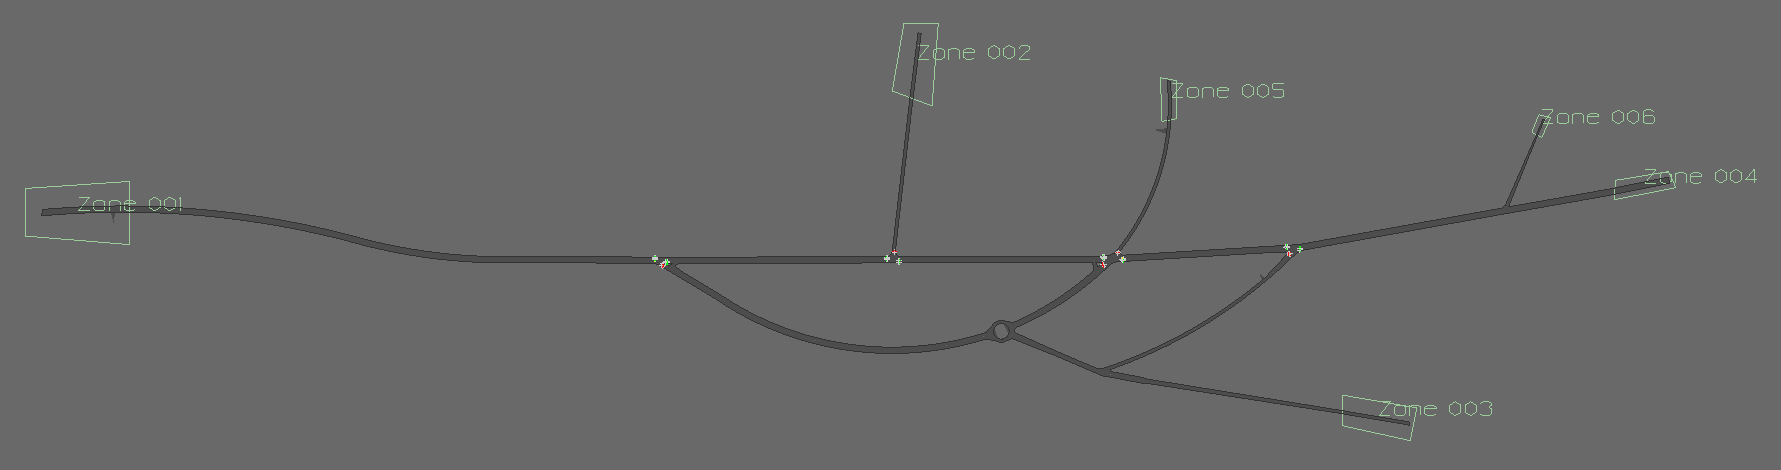
\includegraphics[width=\linewidth]{figuras/network8.png}
    \caption{Red de transporte utilizada para las pruebas preliminares.}
    \label{fig:network8}
\end{figure}

La validación preliminar del \emph{framework} se realizó utilizando la implementación de TraCI en Python incluída en la distribución de SUMO. Esta consiste en una librería para Python 2.7+ y 3.0+, la cual implementa un cliente TraCI en su totalidad (\autocite{pytraci, pytracisrc}), permitiendo así la validación del correcto funcionamiento de los comandos implementados en el \emph{framework} PVeins.

Por otro lado, la red de transporte utilizada para las pruebas corresponde a una red simple, incluida por defecto en la instalación de Paramics. Esta red consiste en un corredor central y conjunto de calles que lo intersectan (ver figura \ref{fig:network8}). El flujo de vehículos en la red es medio-bajo, manteniéndose bajo los 500 vehículos activos en toda la red en cualquier momento dado.

A lo largo del desarrollo de este trabajo, se utilizó la librería anteriormente mencionada, junto con el entorno de \emph{debugging} de Visual Studio y la red de transporte, para probar la correcta implementación de cada funcionalidad que se le agregó al \emph{framework}. Se implementaron simples \emph{scripts} en Python para probar cada una de las funcionalidades desarrolladas; sólo se utilizará uno de éstos como ejemplo a continuación, ya que no es factible ni interesante exponer todas las pruebas realizadas en este documento, dada la gran cantidad de éstas que se efectuaron y el alto grado de similitud que existe entre las mismas.

Además, implementado ya el \emph{framework} en su totalidad, se realizaron pruebas de validación de mayor envergadura, midiendo la eficiencia y la efectividad del sistema para la simulación de grandes redes de transporte. Los resultados de éstas pruebas se presentan en el capítulo \ref{cap:validacion}.

\subsection{Ejemplo de script de prueba: cambio de ruta}

\begin{figure}
    \centering
    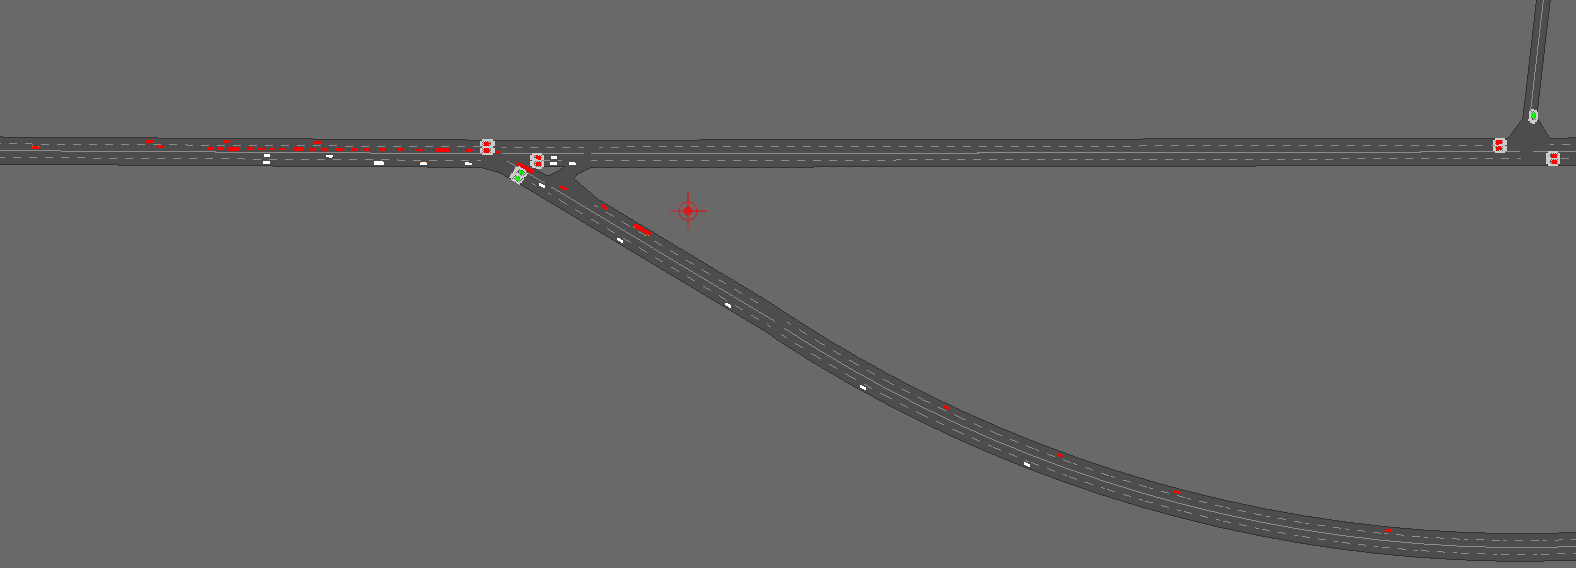
\includegraphics[width=\linewidth]{figuras/network8_routechange.png}
    \caption{Visualización del \emph{test} de cambio de ruta en curso. Los vehículos pintados de rojo son aquellos afectados por el cambio.}
    \label{fig:network8:routechange}
\end{figure}

El código \ref{code:py_routechange} expone el \emph{script} utilizado para una prueba de la funcionalidad del cambio de ruta en TraCI, la cual fue implementada en la última etapa de desarrollo del software por lo que ya se contaba con una base con más funcionalidades sobre la cual construir (\emph{e.g.}, obtención de valores mediante suscripciones).

El procedimiento es simple; el \emph{script} avanza la simulación en un \emph{loop}, obteniendo luego de cada iteración la lista de vehículos en la red. De estos vehículos, encuentra aquellos que se encuentran en la primera calle de una ruta predefinida y procede a cambiar su ruta original por una nueva, al mismo tiempo pintándolos de un color rojo para poder distinguirlos del resto. El resultado puede observarse en la figura \ref{fig:network8:routechange}.

Este código expone de manera clara la estructura del \emph{loop} de simulación TraCI, estructura que se replica en VEINS (aunque de manera mucho más compleja); el cliente es quien controla la ejecución de los pasos de simulación, avanzando el escenario a medida que va realizando sus propios cálculos y análisis. También demuestra las razones por la cual se llevó a cabo el desarrollo en etapas comentado en la sección \ref{sec:metodologia} -- si bien el enfoque de esta prueba es la funcionalidad de cambio de ruta, es necesario también el uso de otras funcionalidades de TraCI como el \emph{handshake} de inicio de conexión (\texttt{traci.init(\dots)}), la suscripción a variables de vehículo (\texttt{traci.vehicle.subscribe(\dots)} y \texttt{.getSubscriptionResults(\dots)}), el avance de la simulación (\texttt{traci.simulationStep()}) y la obtención de variables de vehículo (\texttt{traci.getRoadID(\dots)}).

\begin{figure*}
    \begin{minipage}{\linewidth}
        \lstinputlisting[style=MyPython, caption={\emph{Script} para la prueba de cambio de ruta.}, label={code:py_routechange}]{codigo/pytraci_routechange.py}
    \end{minipage}
\end{figure*}

